\documentclass[10pt,twoside]{article}
\usepackage{graphicx}
\usepackage{url}

\newcommand{\doctitle}{%
Sudoku Solver}
\newcommand{\cmnt}[1]{}

\pagestyle{myheadings}
\markboth{\hfill\doctitle}{\doctitle\hfill}

\bibliographystyle{siam}

\addtolength{\textwidth}{1.00in}
\addtolength{\textheight}{1.00in}
\addtolength{\evensidemargin}{-1.00in}
\addtolength{\oddsidemargin}{-0.00in}
\addtolength{\topmargin}{-.50in}

\hyphenation{in-de-pen-dent}

%\title{\textbf{\doctitle}\\
\title{\textbf{ CS598 Project Proposal: Parallel Sudoku Solver}}

\author{Sandeep Dasgupta\thanks{Electronic address: \texttt{sdasgup3@illinois.edu}}
\qquad Tanmay Gangwani\thanks{Electronic address: \texttt{gangwan2@illinois.edu}}
\qquad  Mengjia Yan\thanks{Electronic address:
\texttt{myan8@illinois.edu}}} 

\begin{document}

\thispagestyle{empty}

\maketitle

  Sudoku puzzles consists of partially filled matrix $N \times N$. The algorithm needs
  to fill the blank positions with values 1 through N such that no number is
  repeated on each of the N rows, N columns or the squares of $\sqrt{N} \times
  \sqrt{N} $ cells that split the original matrix.  The goal will be to solve
  the grid in the least possible time using the parallelization model provided by Charm++.

  Sudoku is an NP-complete problem. The solution space rapidly explodes as we move to 
  higher grid dimensions. For example, it has been proven that the total number of
  valid Sudoku grids, for $N = 9$,  is $6,670,903,752,021,072,936,960$ or
  approximately $6.671 \times 10^{21}$. This precludes using brute force techniques. We would 
  investigate heuristics based on the "logical' properties of Sudoku to reduce the search space 
  and optimize the running time of the algorithm. Sudoko solutions are achieved incrementally by 
  solving instances of smaller problems. Updates to one part of the grid may significantly
  impact other parts which leads to a high degree of communication between objects handling the 
  grid. Load imbalance is inherent in the problem since some parts of the grid may be easier to
  proceed with than other. We plan to leverage the Charm++ model to tackle these challenges. In later 
  stages of the project, we may include the use of the Charm checkpointing support for a part of the
  algorithm which guesstimates certain numbers, and backtracks if a dead end is found.

  \begin{figure}[h]
  \centering
    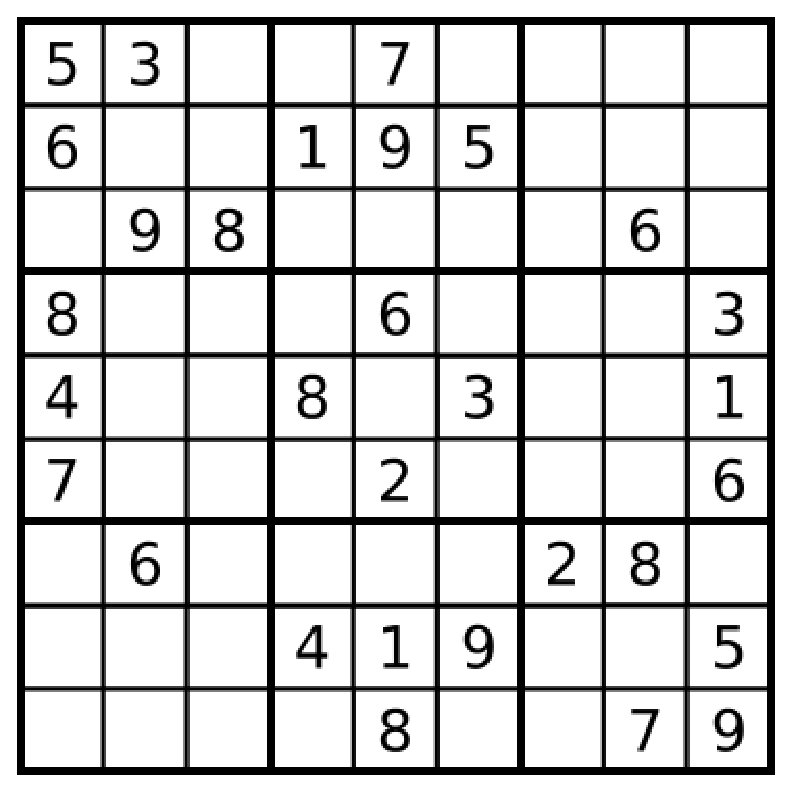
\includegraphics[scale=0.35]{sudoku} 
  \caption{Sudoku Grid} 
  \end{figure}

  




%\nocite{*}
%\bibliography{CS598_project_proposal}

\end{document}
